\documentclass[10pt]{article}
\usepackage[letterpaper,margin=0.75in]{geometry}
\usepackage[T1]{fontenc}
\usepackage{lmodern,graphicx,booktabs,amsmath,array,longtable}
\usepackage{placeins}
\usepackage[hyphens]{url}
\usepackage[numbers,sort&compress]{natbib}
\usepackage[hidelinks]{hyperref}
\setlength{\textfloatsep}{9pt plus 2pt minus 2pt}
\setlength{\floatsep}{7pt plus 2pt minus 2pt}
\setlength{\abovecaptionskip}{5pt}
\setlength{\emergencystretch}{1.5em}
\renewcommand{\topfraction}{0.9}
\renewcommand{\textfraction}{0.07}
\renewcommand{\floatpagefraction}{0.7}
% Generated only from v0.1.0-data. Do not edit empirical values by hand.
\newcommand{\N}[1]{\csname nr@#1\endcsname}
\expandafter\def\csname nr@PilotPinnedLongShort\endcsname{73.724}
\expandafter\def\csname nr@PilotRecomputeLongShort\endcsname{1,737.026}
\expandafter\def\csname nr@ModelCount\endcsname{7}
\expandafter\def\csname nr@T4Timings\endcsname{26,040}
\expandafter\def\csname nr@T4Invalid\endcsname{0}
\expandafter\def\csname nr@T4Sessions\endcsname{10}
\expandafter\def\csname nr@AdjustedCorrect\endcsname{1,237}
\expandafter\def\csname nr@PrefixCorrect\endcsname{1,017}
\expandafter\def\csname nr@T4Resolved\endcsname{1,258}
\expandafter\def\csname nr@L4Correct\endcsname{574}
\expandafter\def\csname nr@L4Resolved\endcsname{636}
\expandafter\def\csname nr@L4Unresolved\endcsname{13}
\expandafter\def\csname nr@L4Cells\endcsname{767}
\expandafter\def\csname nr@L4MAE\endcsname{3.203}
\expandafter\def\csname nr@A10Correct\endcsname{192}
\expandafter\def\csname nr@A10Resolved\endcsname{206}
\expandafter\def\csname nr@A10Unresolved\endcsname{14}
\expandafter\def\csname nr@A10Cells\endcsname{260}
\expandafter\def\csname nr@A10MAE\endcsname{2.040}
\expandafter\def\csname nr@A10GCorrect\endcsname{398}
\expandafter\def\csname nr@A10GResolved\endcsname{426}
\expandafter\def\csname nr@A10GUnresolved\endcsname{3}
\expandafter\def\csname nr@A10GCells\endcsname{507}
\expandafter\def\csname nr@A10GMAE\endcsname{5.758}
\expandafter\def\csname nr@H100Correct\endcsname{20}
\expandafter\def\csname nr@H100Resolved\endcsname{21}
\expandafter\def\csname nr@H100Unresolved\endcsname{1}
\expandafter\def\csname nr@H100Cells\endcsname{26}
\expandafter\def\csname nr@H100MAE\endcsname{6.579}
\expandafter\def\csname nr@KaggleReads\endcsname{7,762}
\expandafter\def\csname nr@KaggleFileSamples\endcsname{7,762}
\expandafter\def\csname nr@KaggleMinBytes\endcsname{196,608}
\expandafter\def\csname nr@KaggleMaxBytes\endcsname{1,879,052,288}
\expandafter\def\csname nr@ModalReads\endcsname{0}
\expandafter\def\csname nr@ModalFileSamples\endcsname{4,575}
\expandafter\def\csname nr@ModalMinBytes\endcsname{0}
\expandafter\def\csname nr@ModalMaxBytes\endcsname{0}
\expandafter\def\csname nr@HalfPrefix\endcsname{226.626}
\expandafter\def\csname nr@HalfAdjusted\endcsname{2,442.265}
\expandafter\def\csname nr@PythiaLow\endcsname{798.9}
\expandafter\def\csname nr@PythiaHigh\endcsname{1597.2}
\expandafter\def\csname nr@QwenMainLow\endcsname{199.5}
\expandafter\def\csname nr@QwenMainHigh\endcsname{398.4}
\expandafter\def\csname nr@PhiLow\endcsname{799.2}
\expandafter\def\csname nr@PhiHigh\endcsname{1598.4}
\expandafter\def\csname nr@QwenThreeLow\endcsname{99.9}
\expandafter\def\csname nr@QwenThreeHigh\endcsname{199.7}
\expandafter\def\csname nr@A10GExtrapPred\endcsname{8,041.096}
\expandafter\def\csname nr@A10GExtrapObs\endcsname{13,914.555}
\expandafter\def\csname nr@A10GExtrapError\endcsname{5,873.459}
\expandafter\def\csname nr@L4ExtrapPred\endcsname{13,088.360}
\expandafter\def\csname nr@L4ExtrapObs\endcsname{18,022.902}
\expandafter\def\csname nr@L4ExtrapError\endcsname{4,934.542}
\expandafter\def\csname nr@T4SpreadShort\endcsname{12.341}
\expandafter\def\csname nr@T4SpreadLong\endcsname{14.847}
\expandafter\def\csname nr@L4SpreadShort\endcsname{4.956}
\expandafter\def\csname nr@L4SpreadLong\endcsname{4.417}
\expandafter\def\csname nr@AmpereSpreadShort\endcsname{23.611}
\expandafter\def\csname nr@AmpereSpreadLong\endcsname{22.664}
\expandafter\def\csname nr@TorchOldError\endcsname{11.78}
\expandafter\def\csname nr@TorchNewError\endcsname{3.097}
\expandafter\def\csname nr@RawOldError\endcsname{3.107}
\expandafter\def\csname nr@RawNewError\endcsname{3.086}
\expandafter\def\csname nr@H100Missing\endcsname{52}
\expandafter\def\csname nr@AnomalyReversals\endcsname{0}
\expandafter\def\csname nr@AnomalyPairs\endcsname{4}
\expandafter\def\csname nr@CalA10Seconds\endcsname{42.5}
\expandafter\def\csname nr@CalL4Seconds\endcsname{63.4}
\expandafter\def\csname nr@L4RatioYes\endcsname{25}
\expandafter\def\csname nr@L4RatioTotal\endcsname{27}
\expandafter\def\csname nr@L4RatioUnresolved\endcsname{32}
\expandafter\def\csname nr@A10RatioYes\endcsname{11}
\expandafter\def\csname nr@A10RatioTotal\endcsname{12}
\expandafter\def\csname nr@A10RatioUnresolved\endcsname{8}
\expandafter\def\csname nr@A10GRatioYes\endcsname{20}
\expandafter\def\csname nr@A10GRatioTotal\endcsname{24}
\expandafter\def\csname nr@A10GRatioUnresolved\endcsname{15}
\expandafter\def\csname nr@H100RatioYes\endcsname{0}
\expandafter\def\csname nr@H100RatioTotal\endcsname{1}
\expandafter\def\csname nr@H100RatioUnresolved\endcsname{1}
\expandafter\def\csname nr@T4Held2Correct\endcsname{148}
\expandafter\def\csname nr@T4Held2Resolved\endcsname{149}
\expandafter\def\csname nr@T4Held3Correct\endcsname{146}
\expandafter\def\csname nr@T4Held3Resolved\endcsname{150}
\expandafter\def\csname nr@Short\endcsname{32}
\expandafter\def\csname nr@Long\endcsname{256}
\expandafter\def\csname nr@Tiny\endcsname{16}
\expandafter\def\csname nr@Small\endcsname{64}
\expandafter\def\csname nr@Mid\endcsname{128}
\expandafter\def\csname nr@Boundary\endcsname{256}
\expandafter\def\csname nr@Example\endcsname{512}
\expandafter\def\csname nr@Matched\endcsname{1,024}
\expandafter\def\csname nr@LongPrefix\endcsname{8,192}
\expandafter\def\csname nr@MaxMain\endcsname{16,384}
\expandafter\def\csname nr@ExtrapLength\endcsname{32,736}
\expandafter\def\csname nr@FullRepeats\endcsname{10}
\expandafter\def\csname nr@CalRepeats\endcsname{3}
\expandafter\def\csname nr@MicroRepeats\endcsname{5}
\expandafter\def\csname nr@Warmups\endcsname{1}
\expandafter\def\csname nr@Bootstraps\endcsname{10,000}
\expandafter\def\csname nr@CI\endcsname{95}
\expandafter\def\csname nr@SessionsT4\endcsname{3}
\expandafter\def\csname nr@SessionsL4\endcsname{2}
\expandafter\def\csname nr@RateLow\endcsname{50}
\expandafter\def\csname nr@RateHigh\endcsname{1,600}
\expandafter\def\csname nr@Rates\endcsname{50, 100, 200, 400, 800, 1,600}
\expandafter\def\csname nr@Rate100\endcsname{100}
\expandafter\def\csname nr@Rate200\endcsname{200}
\expandafter\def\csname nr@Rate400\endcsname{400}
\expandafter\def\csname nr@Rate800\endcsname{800}
\expandafter\def\csname nr@Rate1600\endcsname{1,600}
\expandafter\def\csname nr@PilotMid\endcsname{2,048}
\expandafter\def\csname nr@PilotRepeats\endcsname{12}
\expandafter\def\csname nr@AmpereGeneration\endcsname{4}
\expandafter\def\csname nr@MainGrid\endcsname{16, 64, 128, 256, 512, 1,024, 2,048, 4,096, 8,192, 16,384}
\expandafter\def\csname nr@ShortGrid\endcsname{16, 64, 128, 256}
\expandafter\def\csname nr@MhaGrid\endcsname{64, 256, 512, 1,024}
\expandafter\def\csname nr@KV0\endcsname{12,288}
\expandafter\def\csname nr@KV1\endcsname{28,672}
\expandafter\def\csname nr@KV2\endcsname{36,864}
\expandafter\def\csname nr@KV3\endcsname{196,608}
\expandafter\def\csname nr@KV4\endcsname{196,608}
\expandafter\def\csname nr@KV5\endcsname{327,680}
\expandafter\def\csname nr@KV6\endcsname{114,688}
\expandafter\def\csname nr@Cov0Turn\endcsname{32}
\expandafter\def\csname nr@Cov0Prefixes\endcsname{16, 32, 64, 128, 256, 512, 1,024, 1,792}
\expandafter\def\csname nr@Cov0Sessions\endcsname{1}
\expandafter\def\csname nr@Cov1Turn\endcsname{256}
\expandafter\def\csname nr@Cov1Prefixes\endcsname{16, 32, 64, 128, 256, 512, 1,024, 1,792}
\expandafter\def\csname nr@Cov1Sessions\endcsname{1}
\expandafter\def\csname nr@Cov2Turn\endcsname{32}
\expandafter\def\csname nr@Cov2Prefixes\endcsname{16, 32, 64, 128, 256, 512, 1,024, 2,048, 4,096, 8,192}
\expandafter\def\csname nr@Cov2Sessions\endcsname{1}
\expandafter\def\csname nr@Cov3Turn\endcsname{256}
\expandafter\def\csname nr@Cov3Prefixes\endcsname{16, 32, 64, 128, 256, 512, 1,024, 2,048, 4,096, 8,192}
\expandafter\def\csname nr@Cov3Sessions\endcsname{1}
\expandafter\def\csname nr@Cov4Turn\endcsname{32}
\expandafter\def\csname nr@Cov4Prefixes\endcsname{16, 32, 64, 128, 256, 512, 1,024, 1,792, 2,048, 8,192}
\expandafter\def\csname nr@Cov4Sessions\endcsname{1}
\expandafter\def\csname nr@Cov5Turn\endcsname{32}
\expandafter\def\csname nr@Cov5Prefixes\endcsname{16, 32, 64, 128, 256, 512, 1,024, 2,048, 4,096, 8,192, 16,384}
\expandafter\def\csname nr@Cov5Sessions\endcsname{3}
\expandafter\def\csname nr@Cov6Turn\endcsname{256}
\expandafter\def\csname nr@Cov6Prefixes\endcsname{16, 32, 64, 128, 256, 512, 1,024, 2,048, 4,096, 8,192, 16,384}
\expandafter\def\csname nr@Cov6Sessions\endcsname{3}
\expandafter\def\csname nr@Cov7Turn\endcsname{32}
\expandafter\def\csname nr@Cov7Prefixes\endcsname{16, 32, 64, 128, 256, 512, 1,024, 2,048, 4,096, 8,192, 16,384}
\expandafter\def\csname nr@Cov7Sessions\endcsname{1}
\expandafter\def\csname nr@Cov8Turn\endcsname{256}
\expandafter\def\csname nr@Cov8Prefixes\endcsname{16, 32, 64, 128, 256, 512, 1,024, 2,048, 4,096, 8,192, 16,384}
\expandafter\def\csname nr@Cov8Sessions\endcsname{1}
\expandafter\def\csname nr@Cov9Turn\endcsname{32}
\expandafter\def\csname nr@Cov9Prefixes\endcsname{16, 32, 64, 128, 256, 512, 1,024}
\expandafter\def\csname nr@Cov9Sessions\endcsname{1}
\expandafter\def\csname nr@Cov10Turn\endcsname{256}
\expandafter\def\csname nr@Cov10Prefixes\endcsname{16, 32, 64, 128, 256, 512, 1,024}
\expandafter\def\csname nr@Cov10Sessions\endcsname{1}
\expandafter\def\csname nr@Cov11Turn\endcsname{32}
\expandafter\def\csname nr@Cov11Prefixes\endcsname{16, 32, 64, 128, 256, 512, 1,024, 1,792}
\expandafter\def\csname nr@Cov11Sessions\endcsname{1}
\expandafter\def\csname nr@Cov12Turn\endcsname{256}
\expandafter\def\csname nr@Cov12Prefixes\endcsname{16, 32, 64, 128, 256, 512, 1,024, 1,792}
\expandafter\def\csname nr@Cov12Sessions\endcsname{1}
\expandafter\def\csname nr@Cov13Turn\endcsname{32}
\expandafter\def\csname nr@Cov13Prefixes\endcsname{16, 32, 64, 128, 256, 512, 1,024, 2,048, 4,096, 8,192, 16,384}
\expandafter\def\csname nr@Cov13Sessions\endcsname{1}
\expandafter\def\csname nr@Cov14Turn\endcsname{256}
\expandafter\def\csname nr@Cov14Prefixes\endcsname{16, 32, 64, 128, 256, 512, 1,024, 2,048, 4,096, 8,192, 16,384}
\expandafter\def\csname nr@Cov14Sessions\endcsname{1}
\expandafter\def\csname nr@Cov15Turn\endcsname{32}
\expandafter\def\csname nr@Cov15Prefixes\endcsname{16, 64, 128, 256, 512, 1,024, 2,048, 4,096, 8,192, 16,384}
\expandafter\def\csname nr@Cov15Sessions\endcsname{1}
\expandafter\def\csname nr@Cov16Turn\endcsname{256}
\expandafter\def\csname nr@Cov16Prefixes\endcsname{16, 64, 128, 256, 512, 1,024, 2,048, 4,096, 8,192, 16,384}
\expandafter\def\csname nr@Cov16Sessions\endcsname{1}
\expandafter\def\csname nr@Cov17Turn\endcsname{32}
\expandafter\def\csname nr@Cov17Prefixes\endcsname{64, 256, 512, 1,024, 2,016}
\expandafter\def\csname nr@Cov17Sessions\endcsname{1}
\expandafter\def\csname nr@Cov18Turn\endcsname{32}
\expandafter\def\csname nr@Cov18Prefixes\endcsname{16, 64, 128, 256, 512, 1,024, 2,048, 4,096, 8,192, 16,384}
\expandafter\def\csname nr@Cov18Sessions\endcsname{1}
\expandafter\def\csname nr@Cov19Turn\endcsname{256}
\expandafter\def\csname nr@Cov19Prefixes\endcsname{16, 64, 128, 256, 512, 1,024, 2,048, 4,096, 8,192, 16,384}
\expandafter\def\csname nr@Cov19Sessions\endcsname{1}
\expandafter\def\csname nr@Cov20Turn\endcsname{32}
\expandafter\def\csname nr@Cov20Prefixes\endcsname{64, 256, 512, 1,024, 32,736}
\expandafter\def\csname nr@Cov20Sessions\endcsname{1}
\expandafter\def\csname nr@Cov21Turn\endcsname{32}
\expandafter\def\csname nr@Cov21Prefixes\endcsname{64, 256, 512, 1,024, 2,016}
\expandafter\def\csname nr@Cov21Sessions\endcsname{1}
\expandafter\def\csname nr@Cov22Turn\endcsname{32}
\expandafter\def\csname nr@Cov22Prefixes\endcsname{64, 256, 512, 1,024}
\expandafter\def\csname nr@Cov22Sessions\endcsname{1}
\expandafter\def\csname nr@Cov23Turn\endcsname{32}
\expandafter\def\csname nr@Cov23Prefixes\endcsname{1,024, 16,384}
\expandafter\def\csname nr@Cov23Sessions\endcsname{1}
\expandafter\def\csname nr@Cov24Turn\endcsname{32}
\expandafter\def\csname nr@Cov24Prefixes\endcsname{64, 256, 512, 1,024, 2,016}
\expandafter\def\csname nr@Cov24Sessions\endcsname{1}
\expandafter\def\csname nr@Cov25Turn\endcsname{32}
\expandafter\def\csname nr@Cov25Prefixes\endcsname{16, 64, 128, 256, 512, 1,024, 2,048, 4,096, 8,192, 16,384}
\expandafter\def\csname nr@Cov25Sessions\endcsname{2}
\expandafter\def\csname nr@Cov26Turn\endcsname{256}
\expandafter\def\csname nr@Cov26Prefixes\endcsname{16, 64, 128, 256, 512, 1,024, 2,048, 4,096, 8,192, 16,384}
\expandafter\def\csname nr@Cov26Sessions\endcsname{2}
\expandafter\def\csname nr@Cov27Turn\endcsname{32}
\expandafter\def\csname nr@Cov27Prefixes\endcsname{64, 256, 512, 1,024, 32,736}
\expandafter\def\csname nr@Cov27Sessions\endcsname{1}
\expandafter\def\csname nr@Cov28Turn\endcsname{32}
\expandafter\def\csname nr@Cov28Prefixes\endcsname{64, 256, 512, 1,024, 2,016}
\expandafter\def\csname nr@Cov28Sessions\endcsname{1}
\expandafter\def\csname nr@Cov29Turn\endcsname{32}
\expandafter\def\csname nr@Cov29Prefixes\endcsname{64, 256, 512, 1,024}
\expandafter\def\csname nr@Cov29Sessions\endcsname{1}
\expandafter\def\csname nr@Cov30Turn\endcsname{32}
\expandafter\def\csname nr@Cov30Prefixes\endcsname{512, 2,048, 8,192}
\expandafter\def\csname nr@Cov30Sessions\endcsname{1}
\expandafter\def\csname nr@Cov31Turn\endcsname{256}
\expandafter\def\csname nr@Cov31Prefixes\endcsname{512, 2,048, 8,192}
\expandafter\def\csname nr@Cov31Sessions\endcsname{1}
\expandafter\def\csname nr@Score12Col2\endcsname{574 / 636}
\expandafter\def\csname nr@Score12Col3\endcsname{13}
\expandafter\def\csname nr@Score12Col4\endcsname{767}
\expandafter\def\csname nr@Score12Col5\endcsname{3.203}
\expandafter\def\csname nr@Score13Col2\endcsname{246 / 248}
\expandafter\def\csname nr@Score13Col3\endcsname{5}
\expandafter\def\csname nr@Score13Col4\endcsname{299}
\expandafter\def\csname nr@Score13Col5\endcsname{2.822}
\expandafter\def\csname nr@Score14Col2\endcsname{231 / 289}
\expandafter\def\csname nr@Score14Col3\endcsname{8}
\expandafter\def\csname nr@Score14Col4\endcsname{351}
\expandafter\def\csname nr@Score14Col5\endcsname{2.981}
\expandafter\def\csname nr@Score15Col2\endcsname{97 / 99}
\expandafter\def\csname nr@Score15Col3\endcsname{0}
\expandafter\def\csname nr@Score15Col4\endcsname{117}
\expandafter\def\csname nr@Score15Col5\endcsname{4.007}
\expandafter\def\csname nr@Score16Col2\endcsname{193 / 201}
\expandafter\def\csname nr@Score16Col3\endcsname{8}
\expandafter\def\csname nr@Score16Col4\endcsname{247}
\expandafter\def\csname nr@Score16Col5\endcsname{1.506}
\expandafter\def\csname nr@Score17Col2\endcsname{188 / 216}
\expandafter\def\csname nr@Score17Col3\endcsname{4}
\expandafter\def\csname nr@Score17Col4\endcsname{260}
\expandafter\def\csname nr@Score17Col5\endcsname{3.681}
\expandafter\def\csname nr@Score18Col2\endcsname{193 / 219}
\expandafter\def\csname nr@Score18Col3\endcsname{1}
\expandafter\def\csname nr@Score18Col4\endcsname{260}
\expandafter\def\csname nr@Score18Col5\endcsname{3.654}
\expandafter\def\csname nr@Score19Col2\endcsname{192 / 206}
\expandafter\def\csname nr@Score19Col3\endcsname{14}
\expandafter\def\csname nr@Score19Col4\endcsname{260}
\expandafter\def\csname nr@Score19Col5\endcsname{2.040}
\expandafter\def\csname nr@Score20Col2\endcsname{59 / 63}
\expandafter\def\csname nr@Score20Col3\endcsname{3}
\expandafter\def\csname nr@Score20Col4\endcsname{78}
\expandafter\def\csname nr@Score20Col5\endcsname{2.275}
\expandafter\def\csname nr@Score21Col2\endcsname{96 / 105}
\expandafter\def\csname nr@Score21Col3\endcsname{5}
\expandafter\def\csname nr@Score21Col4\endcsname{130}
\expandafter\def\csname nr@Score21Col5\endcsname{2.308}
\expandafter\def\csname nr@Score22Col2\endcsname{37 / 38}
\expandafter\def\csname nr@Score22Col3\endcsname{6}
\expandafter\def\csname nr@Score22Col4\endcsname{52}
\expandafter\def\csname nr@Score22Col5\endcsname{1.341}
\expandafter\def\csname nr@Score23Col2\endcsname{192 / 206}
\expandafter\def\csname nr@Score23Col3\endcsname{14}
\expandafter\def\csname nr@Score23Col4\endcsname{260}
\expandafter\def\csname nr@Score23Col5\endcsname{2.040}
\expandafter\def\csname nr@Score24Col2\endcsname{398 / 426}
\expandafter\def\csname nr@Score24Col3\endcsname{3}
\expandafter\def\csname nr@Score24Col4\endcsname{507}
\expandafter\def\csname nr@Score24Col5\endcsname{5.758}
\expandafter\def\csname nr@Score25Col2\endcsname{178 / 187}
\expandafter\def\csname nr@Score25Col3\endcsname{0}
\expandafter\def\csname nr@Score25Col4\endcsname{221}
\expandafter\def\csname nr@Score25Col5\endcsname{5.094}
\expandafter\def\csname nr@Score26Col2\endcsname{170 / 185}
\expandafter\def\csname nr@Score26Col3\endcsname{2}
\expandafter\def\csname nr@Score26Col4\endcsname{221}
\expandafter\def\csname nr@Score26Col5\endcsname{5.511}
\expandafter\def\csname nr@Score27Col2\endcsname{50 / 54}
\expandafter\def\csname nr@Score27Col3\endcsname{1}
\expandafter\def\csname nr@Score27Col4\endcsname{65}
\expandafter\def\csname nr@Score27Col5\endcsname{8.371}
\expandafter\def\csname nr@Score28Col2\endcsname{193 / 209}
\expandafter\def\csname nr@Score28Col3\endcsname{0}
\expandafter\def\csname nr@Score28Col4\endcsname{247}
\expandafter\def\csname nr@Score28Col5\endcsname{5.031}
\expandafter\def\csname nr@Score29Col2\endcsname{205 / 217}
\expandafter\def\csname nr@Score29Col3\endcsname{3}
\expandafter\def\csname nr@Score29Col4\endcsname{260}
\expandafter\def\csname nr@Score29Col5\endcsname{6.433}
\expandafter\def\csname nr@Score30Col2\endcsname{20 / 21}
\expandafter\def\csname nr@Score30Col3\endcsname{1}
\expandafter\def\csname nr@Score30Col4\endcsname{26}
\expandafter\def\csname nr@Score30Col5\endcsname{6.579}
\expandafter\def\csname nr@Score31Col2\endcsname{11 / 11}
\expandafter\def\csname nr@Score31Col3\endcsname{0}
\expandafter\def\csname nr@Score31Col4\endcsname{13}
\expandafter\def\csname nr@Score31Col5\endcsname{0.332}
\expandafter\def\csname nr@Score32Col2\endcsname{9 / 10}
\expandafter\def\csname nr@Score32Col3\endcsname{1}
\expandafter\def\csname nr@Score32Col4\endcsname{13}
\expandafter\def\csname nr@Score32Col5\endcsname{9.999}
\expandafter\def\csname nr@Score33Col2\endcsname{20 / 21}
\expandafter\def\csname nr@Score33Col3\endcsname{1}
\expandafter\def\csname nr@Score33Col4\endcsname{26}
\expandafter\def\csname nr@Score33Col5\endcsname{6.579}

% Alternative title: When Is a Cached Conversation Worth Reloading? Measurements Across Commodity GPUs
% Alternative title: The Bandwidth Price of KV Reuse: A Calibrated Study on Older and Commodity GPUs
\title{Reload or Recompute? A Calibrated Rule for KV-Cache Reuse Across Commodity GPUs}
\author{M Mohith\\
\small Chinmaya Vishwa Vidyapeeth, Kochi, India\\
\small\href{mailto:achumohith14@gmail.com}{\nolinkurl{achumohith14@gmail.com}}\\
\small ORCID: \href{https://orcid.org/0009-0003-2978-3045}{0009-0003-2978-3045}}
\date{}
\begin{document}
\maketitle
\begin{abstract}
When a conversation returns, a server must choose whether reloading its key--value (KV) cache or recomputing its prefix gives a faster first token. We evaluate a break-even bandwidth rule for time to first token (TTFT) that includes resident-cache continuation, fixed overhead, and CPU and transfer costs. Building on existing calibration and compute/load analyses, we timestamp and freeze per-cell predictions after short calibration and evaluate separate sweeps on commodity and older GPUs, including short contexts and separate CPU-memory and file paths. Frozen predictions correctly classify \N{L4Correct}/\N{L4Resolved} resolved decisions on L4, \N{A10Correct}/\N{A10Resolved} on A10 x16, and \N{A10GCorrect}/\N{A10GResolved} on A10G x8. For Qwen2.5-1.5B with a \N{Matched}-token prefix and a \N{Short}-token new turn, break-even simulated-bandwidth brackets rise from T4's \N{Rate100}--\N{Rate400} MB/s to \N{Rate800}--\N{Rate1600} MB/s on L4 and A10 x16. Long-context extrapolation can produce large TTFT errors. We release measurements, frozen predictions, reference code, and a source-linked claim ledger.
\end{abstract}
\noindent\textbf{Artifacts:} \href{https://github.com/mohi-devhub/reload-or-recompute}{github.com/mohi-devhub/reload-or-recompute}; frozen release \href{https://github.com/mohi-devhub/reload-or-recompute/releases/tag/v0.1.0-data}{v0.1.0-data}.

\section{Introduction}
In the T4 pilot, Qwen2.5-1.5B returned a first token in a median \N{PilotPinnedLongShort} ms after reloading a pinned CPU cache for an \N{LongPrefix}-token prefix and a \N{Short}-token new turn; recomputing the same input took \N{PilotRecomputeLongShort} ms. When should a server reload a saved conversation cache, and when should it rebuild the prefix? The answer depends on how much time reuse saves after paying for transfer and continuation.

Returning conversations make the choice between reloading a saved prefix and recomputing it a practical latency question for small-model operators on commodity and older GPUs.

py-kvcache already characterizes the reload-versus-recompute trade-off and its hardware dependence, with offline calibration and bandwidth frontiers~\cite{pykvcache}. Cake compares GPUs using simulated I/O bandwidth on MHA and GQA models, and overlaps compute and load~\cite{cake}. We do not claim novelty for KV reuse, offload, break-even thresholds, or choosing compute versus load. Our question is whether a rule fixed during the T4 study can predict later measurements on other GPUs after only short local calibration.

\paragraph{Contributions.}
The first contribution is timestamped, frozen per-cell predictions evaluated on separate sweeps after short local calibration, including GPUs beyond the T4 used to develop the rule. Main-model calibration takes about a minute. Second, we measure commodity and older GPUs and short contexts where reuse costs can outweigh recomputation. Third, we measure CPU-memory and file paths separately, with physical-read observability. The rule's form is fixed before transfer testing; its costs still require calibration.

The reference path measures one request with a saved cache already available. Choosing whether to persist that cache also requires write cost, capacity, and return probability.

\paragraph{Key takeaways.}
\begin{itemize}
\item A short local calibration can predict most reload-versus-recompute choices on a new GPU.
\item Faster prefill can make recomputation preferable for short prefixes and raise the bandwidth needed for reload.
\item Compare the full returning-turn time, and check what the file path actually reads.
\end{itemize}

\section{The TTFT-adjusted decision rule}\label{sec:rule}
Let $L$ be the cached prefix length, $N$ the new-turn length, and $S(L)$ the KV payload in bytes. Let $T_{\mathrm{recompute}}(L,N)$ measure fresh prefill of prefix plus new turn through first-token selection. Let $T_{\mathrm{GPU\,hit}}(L,N)$ measure continuation when the prefix cache is already resident. For a chosen transfer leg with effective bandwidth $B$, use
\begin{equation}
 \widehat T_{\mathrm{reload}}(L,N;B)
 = \widehat T_{\mathrm{GPU\,hit}}(L,N)+\widehat h
 +\frac{S(L)}{B}+\widehat T_{\mathrm{other}}(L,N).
 \label{eq:reload}
\end{equation}
Here $h$ is fixed overhead, and $T_{\mathrm{other}}$ contains measured CPU or transfer legs not represented by $S/B$. For a file path this may include read and deserialization work, with H2D transfer represented either by $S/B$ or by another measured leg. Costs must be counted once. Direct \texttt{torch.load} and staged byte loading have different CPU paths; their cost models must follow those paths.

Writing $D=\widehat T_{\mathrm{recompute}}-\widehat T_{\mathrm{GPU\,hit}}-\widehat h-\widehat T_{\mathrm{other}}$, the break-even bandwidth is
\begin{equation}
 B^*(L,N)=\frac{S(L)}{
 \widehat T_{\mathrm{recompute}}(L,N)-\widehat T_{\mathrm{GPU\,hit}}(L,N)
 -\widehat h-\widehat T_{\mathrm{other}}(L,N)},\qquad D>0.
 \label{eq:bstar}
\end{equation}
For a positive denominator, reload is predicted faster above $B^*$. If the denominator is nonpositive, the additive model predicts no finite bandwidth at which that path wins. This is a model decision, not proof that every implementation must lose. Near a zero denominator, small baseline errors cause large threshold errors; we retain uncertainty rather than force a finite crossing.

A prefix-only approximation compares $S/B$ with prefix prefill alone:
\begin{equation}
 B^*_{\mathrm{prefix}}(L)
 =\frac{S(L)}{T_{\mathrm{prefill}}(L)}
 = k_{\mathrm{KV}}\,r_{\mathrm{prefill}}(L),
 \label{eq:prefix}
\end{equation}
where $k_{\mathrm{KV}}$ is bytes per token and $r_{\mathrm{prefill}}$ is measured prefix tokens per second. This approximation helps explain the bandwidth axis. It does not account for the resumed-turn baseline, buffer creation, tensor views, or CPU work. In particular, reusing a short prefix can leave too little saved time to pay those costs.

The rule has two tests. The T4 redesign evaluates descriptive agreement with measured same-session recompute and resident-hit baselines. Cross-GPU transfer instead predicts those baselines and transfer legs from calibration, freezes the predictions, and scores later sweeps. The latter additionally tests baseline prediction and variation between GPU instances.

\section{Setup and measurement protocol}\label{sec:setup}
\subsection{Three phases and observed hardware}
The pilot tests the main model on T4 at prefixes \N{Example}, \N{PilotMid}, and \N{LongPrefix}, with \N{Short}- and \N{Long}-token turns. The pilot has \N{PilotRepeats} measured repeats per cell; the later sweeps use \N{FullRepeats}. Reload-path medians beat recomputation throughout that pilot grid, so it did not locate a crossover length. The next phase changes the axis to simulated bandwidth and includes short prefixes, multiple model families, separate file legs, and repeated sessions. It contains \N{T4Timings} accepted full-sweep timings, \N{T4Invalid} invalid full-sweep timings, and \N{T4Sessions} sweep sessions across \N{ModelCount} models.

The transfer phase uses L4 and Modal's Ampere allocation tier. The observed boards differ: A10 has an active PCIe generation-\N{AmpereGeneration} x16 link, while A10G has generation-\N{AmpereGeneration} x8. We use A10 calibration, transferred unchanged to A10 and A10G. Their spread is confounded by board, host, and link differences; each board has one main-model session. T4 has \N{SessionsT4} main-model sessions and L4 has \N{SessionsL4}, so their observed ranges do not establish relative platform stability. H100 contributes only complete cells from an interrupted optional GPU instance.

All measured weights and caches use fp16. The transfer runs pin Torch \texttt{2.11.0+cu130} and Transformers \texttt{4.51.3} to the T4 redesign versions. Python patch versions and GPU drivers differ between platforms. The efficient/math SDPA selection is fixed, without the I/O-aware FlashAttention algorithm~\citep{flashattention}. Source hashes protect the timing, forward, continuation, transfer, and file-read routines against changes from the T4 reference. Platform wrappers change GPU checks, scheduling, and persistence, not those protected routines. The reference uses PyTorch~\citep{pytorch} and Transformers~\citep{transformers}; analysis and figures use NumPy~\citep{numpy} and Matplotlib~\citep{matplotlib}.

\subsection{Models, workloads, and coverage}
Table~\ref{tab:models} lists the measured checkpoints and verified cache sizes. The formula for fp16 KV bytes per token counts keys and values, layers, KV heads, head dimension, and bytes per element. Configuration sizes are checked against the tensors; GQA shares KV heads across query heads~\citep{gqa}. Family reports cover Qwen2.5~\citep{qwen}, Pythia~\citep{pythia}, OPT~\citep{opt}, and Llama~\citep{llama}; Table~\ref{tab:models} identifies the actual checkpoints.
\begin{table}[t]
\centering\small
\begin{tabular}{llr}
\toprule Checkpoint & Layout & KV bytes/token \\ \midrule
\path{Qwen/Qwen2.5-0.5B} & GQA & \N{KV0} \\
\path{Qwen/Qwen2.5-1.5B} & GQA & \N{KV1} \\
\path{Qwen/Qwen2.5-3B} & GQA & \N{KV2} \\
\path{EleutherAI/pythia-1.4b} & MHA & \N{KV3} \\
\path{facebook/opt-1.3b} & MHA & \N{KV4} \\
\path{microsoft/phi-2} & MHA & \N{KV5} \\
\path{unsloth/Llama-3.2-3B-Instruct} & GQA & \N{KV6} \\
\bottomrule
\end{tabular}

\caption{Released fp16 models and verified KV payload. The Llama checkpoint is the ungated mirror. These are different models, not a controlled attention-layout intervention.}\label{tab:models}
\end{table}

The main model uses a frozen synthetic UltraChat fixture~\citep{ultrachat}, with conversations stitched for long contexts. A new turn is a fixed-length token continuation of clipped role-labelled text, not necessarily a complete message at a dialogue boundary. Repeated text supplies auxiliary-model controls. Neither workload establishes quality or a natural return distribution.

The transfer main-model grid has prefixes \N{MainGrid}, with new turns \N{Short} and \N{Long}. Controls use a \N{Short}-token turn and a smaller repeated-text grid, including native-supported limits where feasible. A10 has main-model measurements only; A10G and L4 also have the controls. Context and memory exclusions remain explicit. Appendix~\ref{app:coverage} gives the full completed coverage, including T4-specific reductions and the incomplete H100 subset. We do not replace missing cells with predicted measurements.

\subsection{Paths and simulated bandwidth}
The reference measures fresh recomputation, a GPU-resident hit, pinned CPU reload, pageable CPU reload, and local file API paths. The raw staged path reads bytes, constructs a CPU tensor view, and copies to GPU. The direct torch path includes deserialization in \texttt{torch.load}. Independent microbenchmarks measure H2D movement and file CPU legs without the new turn. Cache creation, CPU offload, packing, pinning, file writes, tokenization, input-ID placement, request queueing, and network transport are outside returning-turn TTFT.

For the \emph{simulated-bandwidth} paths, a packed fp16 buffer is copied in chunks. Each chunk is synchronized, and a cumulative rate limiter waits for its byte deadline. Targets are \N{Rates} MB/s, plus an unthrottled control. MB/s uses decimal bytes. We record target and achieved rates separately. Buffer creation participates in the pacing budget, and tensor-view work remains inside TTFT; therefore adding an unthrottled overhead intercept is an approximation, especially for short prefixes. This simulates serialized blocking transfer, not physical devices, network latency distributions, or asynchronous pipelines. The unthrottled pinned path is the real pinned-memory control and is counted once.

\subsection{Timing, calibration, and uncertainty}
Full redesign and transfer sweeps use \N{FullRepeats} measured randomized rounds after warmup. Conditions, including prefix-only prefill, are shuffled within each round. CUDA synchronization and events accompany synchronized wall-clock timing; events can include device idle time during host pacing. The endpoint is first-token selection available to the host. Restored-cache continuation consumes the transferred tensors and is checked against the resident-cache continuation and full-recompute first token. This guards against timing a copy that is never used.

Reported within-session intervals use a percentile bootstrap with \N{Bootstraps} resamples and \N{CI}\% coverage. Decision scoring uses a paired-round bootstrap interval for reload-minus-recompute TTFT. We call a decision resolved when that interval identifies one path as faster. Intervals covering zero are excluded from the accuracy denominator. Median absolute TTFT error includes complete baseline and reload cells. Related cells share models, contexts, calibration, and sessions; decision counts are descriptive, not independent Bernoulli trials.

Before each new GPU sweep, calibration measures prefix-only, recompute, and resident-hit baselines at a few lengths, plus independent transfer and file legs. It uses \N{CalRepeats} baseline rounds and \N{MicroRepeats} microbenchmark repeats. Nonnegative quadratic time models predict prefill and recompute; resident-hit and byte-cost legs use nonnegative affine fits. Predictions for every planned cell are committed before its sweep begins. Sweep observations never update coefficients. We distinguish anchors, interpolation, and extrapolation; Appendix~\ref{app:calibration} specifies anchors and path costs.

Separate session medians are retained. Session spread is the range of those medians divided by their median, not a population interval. Telemetry samples SM and memory clocks, temperature, power, and event reasons at about one sample per second; Modal also records PCIe generation and width. Sampling can miss brief trials, and associations with clocks do not establish a latency cause.

\subsection{File-path observability}\label{sec:files}
Kaggle file reads were physical according to process I/O counters: \N{KaggleReads}/\N{KaggleFileSamples} recorded file observations have positive \texttt{physical\_read\_bytes}, ranging from \N{KaggleMinBytes} to \N{KaggleMaxBytes} bytes. These counts include calibration and file microbenchmarks. The counters support reads beyond kernel page-cache hits; they are not physical-device traces and do not identify underlying media or host/storage caches.

Physical reads were not observed on Modal: \N{ModalReads}/\N{ModalFileSamples} file observations have positive physical-read counters. We call this the \emph{local file API path (physical reads not observed)}. Page-cache residency is one interpretation of the zero counters; the cache layer is unverified. Global cache dropping was denied on Kaggle, and per-file eviction advice is advisory on both platforms. Without a cached-versus-uncached ablation, these platforms do not provide equivalent physical-file-read conditions.

\section{Results}\label{sec:results}
\subsection{Short calibration predicts most decisions on new GPUs}
Short calibration predicted most reload-versus-recompute decisions correctly on the tested GPUs.
Figure~\ref{fig:score} shows \N{L4Correct}/\N{L4Resolved} correct resolved decisions on L4, \N{A10Correct}/\N{A10Resolved} on A10 x16, and \N{A10GCorrect}/\N{A10GResolved} on A10G x8. Their median absolute TTFT errors are \N{L4MAE}, \N{A10MAE}, and \N{A10GMAE} ms, with \N{L4Unresolved}, \N{A10Unresolved}, and \N{A10GUnresolved} unresolved decisions. H100 contributes \N{H100Correct}/\N{H100Resolved} correct resolved decisions and \N{H100Unresolved} unresolved decision. Predictions were frozen before these sweeps.
A10 covers the main model only, L4 and A10G also cover the controls, and H100 is partial.
\begin{figure}[t]
\centering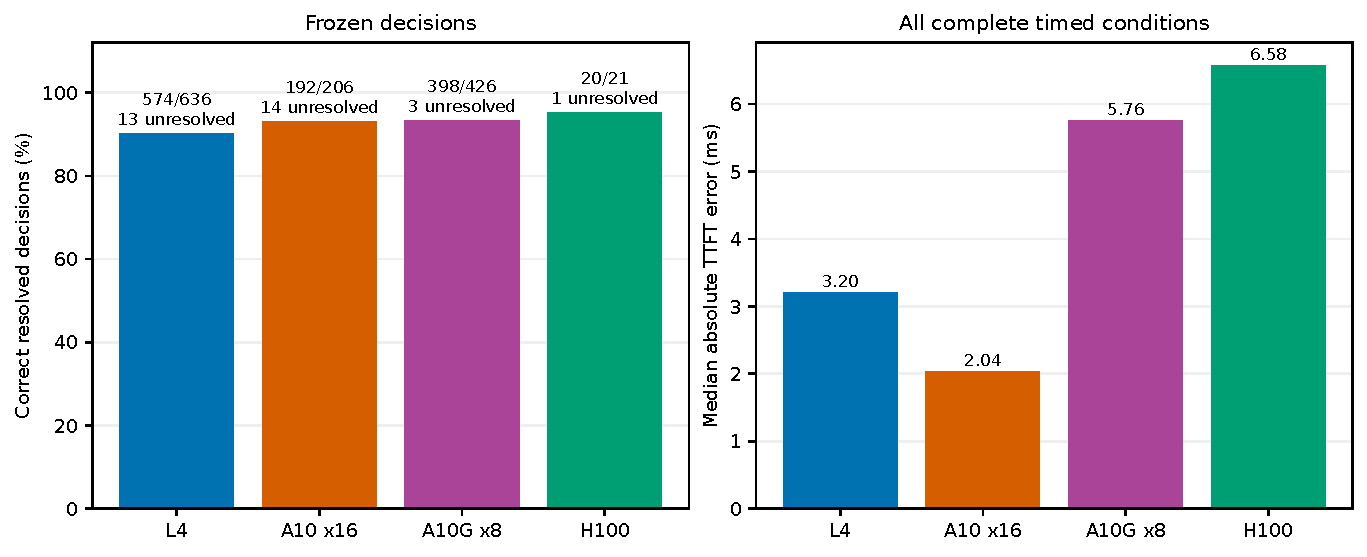
\includegraphics[width=\linewidth]{figures/frozen-scorecard.pdf}
\caption{Frozen decisions and median absolute TTFT errors. Scored decisions compare resident hits and reload paths with recomputation; error includes all complete timed conditions. Coverage is unequal: partial H100 has \N{H100Cells} cells, L4 \N{L4Cells}, A10 x16 \N{A10Cells}, and A10G x8 \N{A10GCells}. A10 covers only the main model. Unresolved decisions are excluded. These bars are not a GPU ranking; Appendix~\ref{app:scores} separates coverage and calibration regions.}\label{fig:score}
\end{figure}

\subsection{Faster GPUs need more bandwidth before reload wins}
The faster GPUs required higher simulated bandwidth before reloading the same prefix became faster than recomputing it.
At main-model prefix \N{Matched} and new turn \N{Short}, the T4 sessions cross between target rates of \N{Rate100}--\N{Rate200} or \N{Rate200}--\N{Rate400} MB/s. L4 and A10 x16 cross between \N{Rate800} and \N{Rate1600} MB/s; A10G x8 crosses between \N{Rate400} and \N{Rate800} MB/s. H100 still favors recomputation at the highest tested rate. Figure~\ref{fig:gpu} shows the individual achieved-rate brackets.
These comparisons use Qwen2.5-1.5B on UltraChat.
\begin{figure}[t]
\centering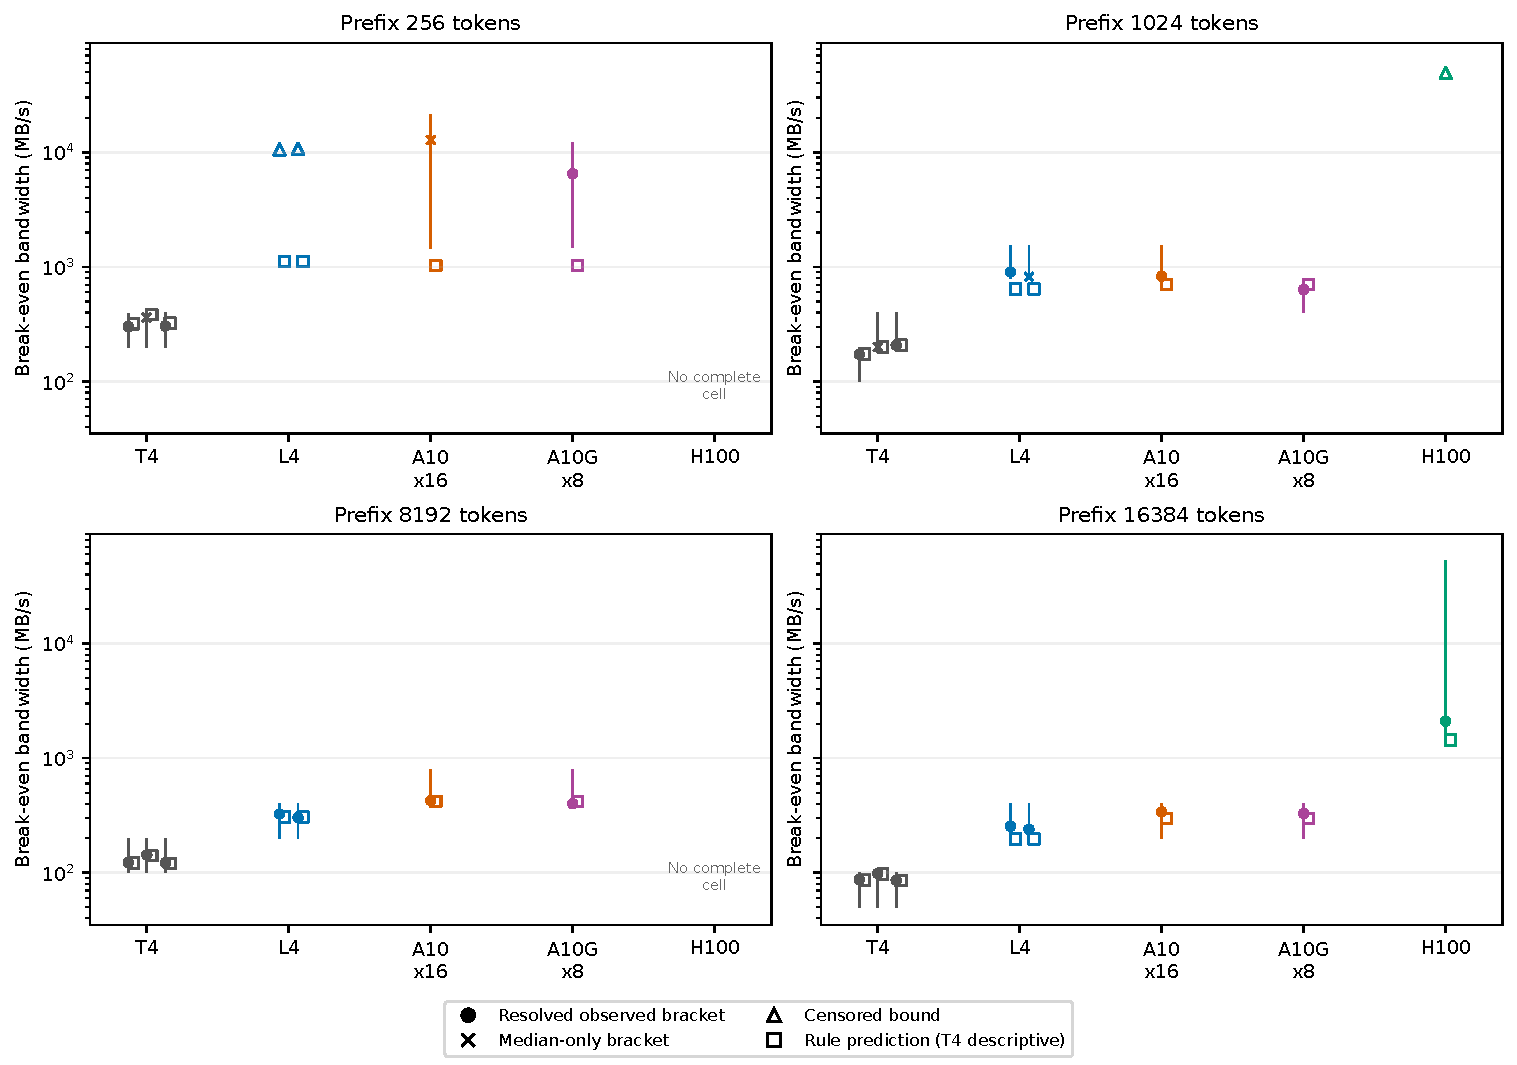
\includegraphics[width=\linewidth]{figures/bstar-vs-gpu.pdf}
\caption{Main-model UltraChat simulated-bandwidth crossovers at matched prefixes, new turn \N{Short}. Bars span achieved-rate endpoints. Circles have resolved endpoints; crosses have an unresolved endpoint. Upward triangles mean recompute faster through the highest tested rate; crossover not located. Squares show the rule, descriptive on T4 and frozen on new GPUs. Sessions remain separate.}\label{fig:gpu}
\end{figure}

\subsection{Returning-turn and fixed costs change the answer}
Including continuation and fixed costs explains decisions that the prefix-only rule misses.
On T4, the adjusted rule agrees with \N{AdjustedCorrect}/\N{T4Resolved} resolved simulated-rate decisions, compared with \N{PrefixCorrect}/\N{T4Resolved} for the prefix-only rule. For Qwen2.5-0.5B at prefix \N{Example} and turn \N{Short}, the prefix-only threshold is \N{HalfPrefix} MB/s, while the adjusted threshold is \N{HalfAdjusted} MB/s; the observed crossing lies between the highest paced rate and the unthrottled control. Fixed first-session calibration predicts later T4 main-model sessions with \N{T4Held2Correct}/\N{T4Held2Resolved} and \N{T4Held3Correct}/\N{T4Held3Resolved} correct resolved decisions.
The rule comparison uses same-session baselines; the later-session check holds the first session's calibration fixed.

\subsection{L4 extends the short-context range where recompute wins}
Recomputation remained faster over more of the sampled short-prefix range on L4 than on T4.
For a \N{Short}-token turn, both L4 sessions favor recomputation at every common prefix in \N{ShortGrid}. T4 favors reload at prefix \N{Boundary} in each session, while smaller prefixes include recompute wins and unresolved comparisons. Figure~\ref{fig:short} shows the sessions for both turn lengths.
These results compare Qwen2.5-1.5B on UltraChat with the real unthrottled pinned-copy path.
\begin{figure}[t]
\centering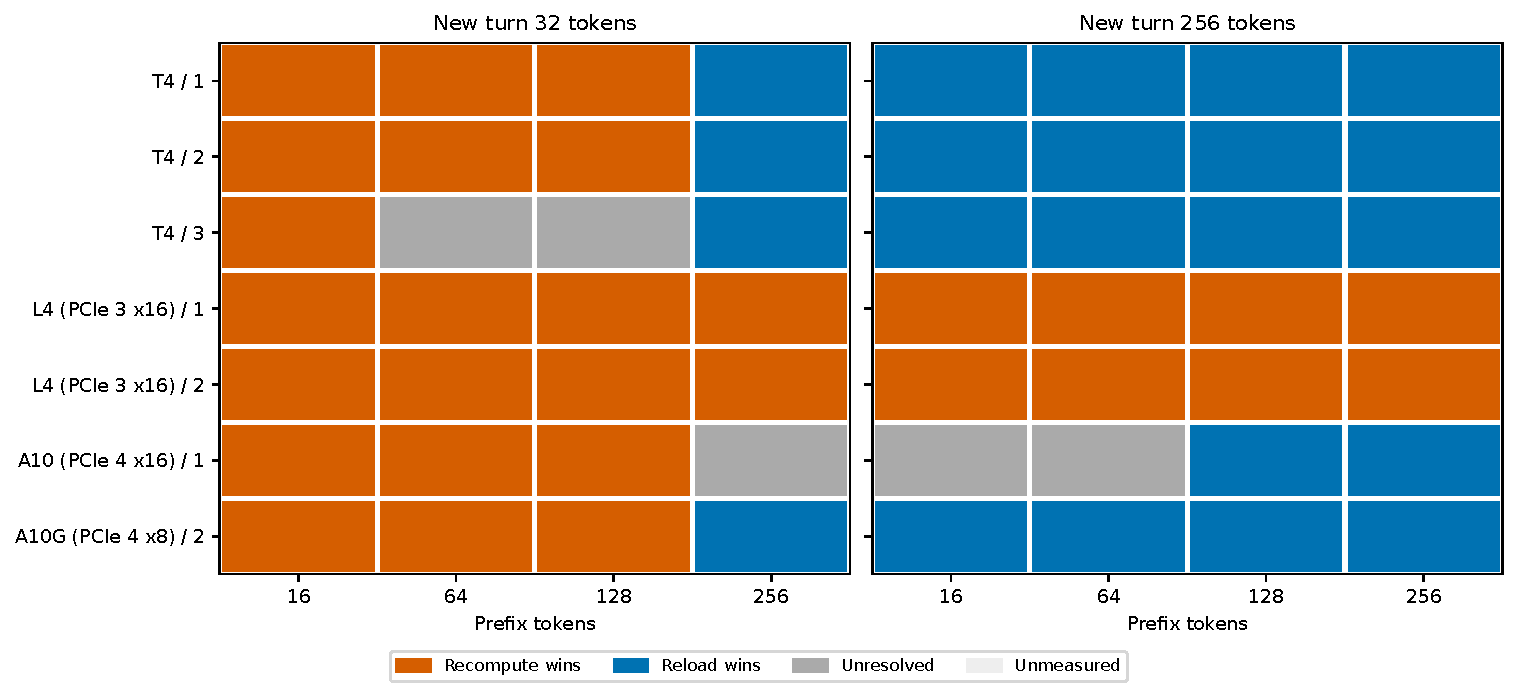
\includegraphics[width=\linewidth]{figures/short-context-regime.pdf}
\caption{Main-model UltraChat choices between recomputation and the real unthrottled pinned-copy path. Rows are separate sessions; panels separate new-turn lengths. Colors follow the paired timing comparison, with unresolved cells shown explicitly.}\label{fig:short}
\end{figure}

\subsection{Supporting model and platform observations}
At matched repeated-text prefix \N{Example} and turn \N{Short} on T4, Pythia's achieved simulated crossover bracket is $[\N{PythiaLow},\N{PythiaHigh}]$ MB/s, with an unresolved endpoint, versus $[\N{QwenMainLow},\N{QwenMainHigh}]$ for Qwen2.5-1.5B. Phi-2's bracket is $[\N{PhiLow},\N{PhiHigh}]$, versus $[\N{QwenThreeLow},\N{QwenThreeHigh}]$ for Qwen2.5-3B. These selected MHA models need higher simulated bandwidth than the selected GQA models. Different parameter counts, prefill kernels, and widths confound an architectural interpretation; we do not estimate a causal effect of GQA.

Including deserialization reduces the T4 torch-file rule's median absolute relative residual from \N{TorchOldError}\% to \N{TorchNewError}\%. The raw-format residual changes only from \N{RawOldError}\% to \N{RawNewError}\%. The correction matters to the relevant CPU path rather than improving every format equally. This residual analysis uses independent file legs and same-session baselines; it is not a new frozen-transfer test.

Recompute session spread also matters. Median relative ranges across lengths are \N{T4SpreadShort}\% and \N{T4SpreadLong}\% on T4 for the short and long turn, versus \N{L4SpreadShort}\% and \N{L4SpreadLong}\% on L4. The A10/A10G relative ranges are \N{AmpereSpreadShort}\% and \N{AmpereSpreadLong}\%; the board and link differences are described in Section~\ref{sec:setup}.

\section{What does not hold}\label{sec:negative}
\paragraph{Long-context extrapolation.}
The low median TTFT errors conceal large native-limit failures. For Qwen2.5-3B at prefix \N{ExtrapLength} with turn \N{Short}, A10G predicts \N{A10GExtrapPred} ms recompute but observes \N{A10GExtrapObs} ms, an absolute error of \N{A10GExtrapError} ms. L4 predicts \N{L4ExtrapPred} ms and observes \N{L4ExtrapObs} ms, an error of \N{L4ExtrapError} ms. A short nonnegative quadratic calibration is therefore not a reliable native-context TTFT predictor for these observations. High decision agreement at other lengths cannot justify that extrapolation.

\paragraph{Exact proportional throughput scaling.}
Figure~\ref{fig:prefill} relates the observed simulated-bandwidth boundary to prefix throughput. The frozen throughput-ratio prediction falls inside at least one matched T4 crossover-ratio bracket for \N{L4RatioYes}/\N{L4RatioTotal} ratio-resolved L4 shapes, \N{A10RatioYes}/\N{A10RatioTotal} A10 shapes, and \N{A10GRatioYes}/\N{A10GRatioTotal} A10G shapes. The partial H100 comparison is \N{H100RatioYes}/\N{H100RatioTotal}. These are broad-bracket compatibility counts, not tests proving equality. Thresholds above the highest tested rate or with unresolved endpoints do not supply exact ratios. The adjusted denominator also changes with continuation and fixed costs. Dividing two prefix-only formula estimates would merely restate an identity, not validate hardware transfer.
\begin{figure}[t]
\centering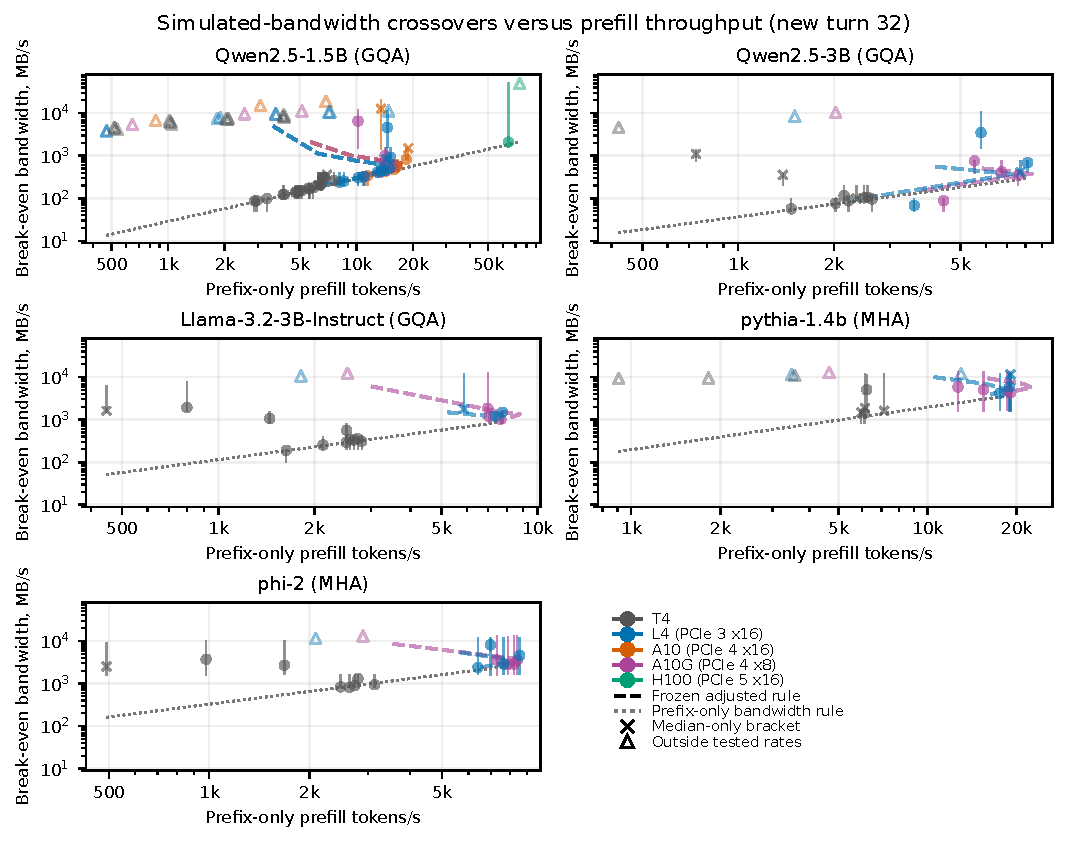
\includegraphics[width=\linewidth]{figures/bstar-vs-prefill.pdf}
\caption{Simulated-bandwidth crossovers and predictions, new turn \N{Short}, five models. Observations use measured prefill throughput; dashed adjusted-rule curves use calibration-predicted throughput, so offsets mix throughput and bandwidth prediction errors. T4 is descriptive; other predictions are frozen. Bars span achieved-rate brackets; crosses have an unresolved endpoint. Upward triangles mean recompute faster through the highest tested rate; crossover not located. Downward triangles mean reload faster down to the lowest tested rate; crossover not located. Dotted lines are KV bytes/token times throughput. Interpolated points are not measured thresholds. Model comparisons are confounded; H100 is partial with no MHA sweep.}\label{fig:prefill}
\end{figure}

\paragraph{Uniform MHA file outcomes.}
On repeated-text, matched prefixes \N{MhaGrid} and a \N{Short}-token turn, Pythia's direct-file path has no resolved reload wins on T4, but wins at a matched prefix on A10G. Phi-2 already has direct-file wins on T4, so a blanket assertion that all MHA file paths lose there is false. Both measured MHA models lose on both L4 file paths. A10 x16 has no MHA sweep. These outcomes do not transfer uniformly, and Section~\ref{sec:files}'s different read conditions prevent attributing the change to GPU speed alone.

\paragraph{The pilot anomaly remains unexplained.}
The pilot's prefix-only median was slower than prefix-plus-turn at the long pilot context. None of the \N{AnomalyPairs} phase-two anomaly comparisons has a positive interval lower endpoint for that reversal. The historical cause was not established. Non-reproduction and randomized ordering improve interpretation, but do not retroactively identify an implementation, clock, or thermal cause.

\section{Practical guidance}\label{sec:guide}
\noindent\fbox{\begin{minipage}{.96\linewidth}
\textbf{A one-minute calibration checklist, not a runtime guarantee.}
After loading and warming the model, measure recompute and resident-hit TTFT at short, typical, and long contexts for the intended turn. Measure pinned/pageable H2D and the file path's CPU read/deserialization legs; check physical-read counters. Apply Equation~\ref{eq:bstar}, counting each leg once, and validate close predictions in paired rounds. Recalibrate after changes to the GPU, link, model, dtype, turn, or file path.

Calibration function times of \N{CalA10Seconds} seconds on A10 and \N{CalL4Seconds} seconds on L4 exclude provider initialization; they do not guarantee this checklist's duration. Near-zero time saved by reuse, untested long contexts, or unknown file-cache state call for more measurement.
\end{minipage}}

The checklist is guidance, not an evaluated deployment. Engine builders must remeasure their actual critical path: buffer preparation, layout, asynchronous copies, and scheduling change it. Overlap scheduling and persistence admission need additional cost models.

\section{Related work}\label{sec:related}
vLLM/PagedAttention manages KV memory and sharing~\citep{vllm}; SGLang's RadixAttention reuses shared prefixes~\citep{sglang}. CachedAttention, earlier named AttentionStore, combines hierarchical multi-turn caching with prefetch and asynchronous saving~\citep{cachedattention}. LMCache provides external KV storage and engine connectors~\citep{lmcache}, while Mooncake disaggregates prefill, decoding, and cache resources~\citep{mooncake}. CacheGen compresses and streams KV~\citep{cachegen}; CacheBlend selectively recomputes cached chunks for fusion~\citep{cacheblend}. Other work examines file-read observability~\citep{fileobservability}, service-aware compression~\citep{kvserve}, and fetching interference~\citep{shadowserve}.

Cake is the closest prior compute/load system: it overlaps computation from the prefix's beginning with loading from its end and compares GPUs using simulated I/O bandwidth on MHA and GQA models~\citep{cake}. Our rule compares load-only and recompute-only endpoints; it does not determine Cake's optimal partial split, and we did not test overlap. py-kvcache already provides offline per-node/model calibration (Section~6.6) and break-even bandwidth frontiers (Section~5.2)~\citep{pykvcache}. This paper is a smaller, reproducible measurement of that break-even on commodity and older GPUs, including short contexts and separate CPU-memory and file paths with read observability. Its distinction is timestamped, frozen per-cell predictions evaluated on separate sweeps after short calibration. We claim no novelty for KV reuse, offload, calibration, or compute-versus-load thresholds.

\section{Limitations and conclusion}\label{sec:limits}
Calibration observes baselines and independent cost legs, not combined reload TTFT. Baseline-fit errors, overhead approximation, and GPU-instance variation therefore remain mixed. The new-GPU tests use local calibration; they are not zero-shot predictions from T4 coefficients. The T4 same-session rule counts are descriptive, while the held-out session check keeps the first session's calibration fixed.

The bandwidth shift and short-context extension describe the observed GPUs rather than an isolated compute effect: host paths, drivers, and links also change. One L4 bandwidth bracket has an unresolved endpoint. A10 and A10G differ at the short-context boundary, and the sampled prefix grid does not locate a continuous crossover length. Decision counts share models, contexts, and calibration, so they are not independent trials. A high aggregate score cannot justify unmeasured contexts. The slower Ampere session did not have lower sampled SM clocks, so those samples alone do not explain its recompute time.

The single-request fp16 reference path establishes neither production-engine performance, multi-request throughput, quantization, bf16, P100 transfer, nor application quality. Production attempts yielded no successful performance observation. Synthetic or repeated text and stitched long inputs do not model a natural return distribution.

Coverage is unequal across boards and model families. H100 has only \N{H100Cells} complete timing cells and \N{H100Missing} unfinished registered cells; only main-model prefixes \N{Matched} and \N{MaxMain} are complete, and its Pythia sweep did not start. Partial records remain in the release but are not scored. One H100 GPU instance cannot establish a general datacenter-GPU or MHA conclusion. Native and memory limits exclude other contexts, and the sparse simulated-rate grid often gives a wide bracket to the unthrottled endpoint.

Frozen-fit uncertainty is not propagated. Within-session intervals and few sessions do not describe a deployment population. File counters identify neither media nor all host caches. Serialized copies do not predict overlap or serving interference. Model differences confound architecture; GPU-instance differences confound causal comparisons.

Within the measured scope, local calibration predicts most resolved decisions. Operators should measure complete returning-turn paths, retain unresolved outcomes, and recalibrate after changes.
\FloatBarrier
\label{main:end}
\clearpage
\label{references:start}
\renewcommand{\refname}{References}
\phantomsection\addcontentsline{toc}{section}{References}
\bibliographystyle{plainnat}
{\small\bibliography{references}}
\clearpage
\appendix
\section{Full completed coverage}\label{app:coverage}
The tables are generated from the immutable release, not a new analysis fit. Full checkpoint identifiers and KV sizes appear in Table~\ref{tab:models}. Phase labels distinguish the pilot, T4 redesign, and transfer. Native-context and budget exclusions are retained; no table entry implies an unmeasured comparison. A10 is PCIe x16, A10G is x8, and their rows are separate.
{\footnotesize\setlength{\tabcolsep}{3pt}\begin{longtable}{p{.78in}p{1.43in}crp{2.55in}r}
\caption{Complete measured coverage. U is UltraChat; R is repeated text. Session counts separate GPU instances, not repeat rounds. Calibration and incomplete H100 cells are excluded.}\label{tab:coverage}\\
\toprule Phase/board & Model & Text & Turn & Prefix tokens & Sessions\\\midrule\endfirsthead
\toprule Phase/board & Model & Text & Turn & Prefix tokens & Sessions\\\midrule\endhead
T4 & pythia-1.4b & R & \N{Cov0Turn} & \N{Cov0Prefixes} & \N{Cov0Sessions} \\
T4 & pythia-1.4b & R & \N{Cov1Turn} & \N{Cov1Prefixes} & \N{Cov1Sessions} \\
T4 & Qwen 0.5B & R & \N{Cov2Turn} & \N{Cov2Prefixes} & \N{Cov2Sessions} \\
T4 & Qwen 0.5B & R & \N{Cov3Turn} & \N{Cov3Prefixes} & \N{Cov3Sessions} \\
T4 & Qwen 1.5B & R & \N{Cov4Turn} & \N{Cov4Prefixes} & \N{Cov4Sessions} \\
T4 & Qwen 1.5B & U & \N{Cov5Turn} & \N{Cov5Prefixes} & \N{Cov5Sessions} \\
T4 & Qwen 1.5B & U & \N{Cov6Turn} & \N{Cov6Prefixes} & \N{Cov6Sessions} \\
T4 & Qwen 3B & R & \N{Cov7Turn} & \N{Cov7Prefixes} & \N{Cov7Sessions} \\
T4 & Qwen 3B & R & \N{Cov8Turn} & \N{Cov8Prefixes} & \N{Cov8Sessions} \\
T4 & opt-1.3b & R & \N{Cov9Turn} & \N{Cov9Prefixes} & \N{Cov9Sessions} \\
T4 & opt-1.3b & R & \N{Cov10Turn} & \N{Cov10Prefixes} & \N{Cov10Sessions} \\
T4 & phi-2 & R & \N{Cov11Turn} & \N{Cov11Prefixes} & \N{Cov11Sessions} \\
T4 & phi-2 & R & \N{Cov12Turn} & \N{Cov12Prefixes} & \N{Cov12Sessions} \\
T4 & Llama 3.2-3B & R & \N{Cov13Turn} & \N{Cov13Prefixes} & \N{Cov13Sessions} \\
T4 & Llama 3.2-3B & R & \N{Cov14Turn} & \N{Cov14Prefixes} & \N{Cov14Sessions} \\
A10 & Qwen 1.5B & U & \N{Cov15Turn} & \N{Cov15Prefixes} & \N{Cov15Sessions} \\
A10 & Qwen 1.5B & U & \N{Cov16Turn} & \N{Cov16Prefixes} & \N{Cov16Sessions} \\
A10G & pythia-1.4b & R & \N{Cov17Turn} & \N{Cov17Prefixes} & \N{Cov17Sessions} \\
A10G & Qwen 1.5B & U & \N{Cov18Turn} & \N{Cov18Prefixes} & \N{Cov18Sessions} \\
A10G & Qwen 1.5B & U & \N{Cov19Turn} & \N{Cov19Prefixes} & \N{Cov19Sessions} \\
A10G & Qwen 3B & R & \N{Cov20Turn} & \N{Cov20Prefixes} & \N{Cov20Sessions} \\
A10G & phi-2 & R & \N{Cov21Turn} & \N{Cov21Prefixes} & \N{Cov21Sessions} \\
A10G & Llama 3.2-3B & R & \N{Cov22Turn} & \N{Cov22Prefixes} & \N{Cov22Sessions} \\
H100 & Qwen 1.5B & U & \N{Cov23Turn} & \N{Cov23Prefixes} & \N{Cov23Sessions} \\
L4 & pythia-1.4b & R & \N{Cov24Turn} & \N{Cov24Prefixes} & \N{Cov24Sessions} \\
L4 & Qwen 1.5B & U & \N{Cov25Turn} & \N{Cov25Prefixes} & \N{Cov25Sessions} \\
L4 & Qwen 1.5B & U & \N{Cov26Turn} & \N{Cov26Prefixes} & \N{Cov26Sessions} \\
L4 & Qwen 3B & R & \N{Cov27Turn} & \N{Cov27Prefixes} & \N{Cov27Sessions} \\
L4 & phi-2 & R & \N{Cov28Turn} & \N{Cov28Prefixes} & \N{Cov28Sessions} \\
L4 & Llama 3.2-3B & R & \N{Cov29Turn} & \N{Cov29Prefixes} & \N{Cov29Sessions} \\
Pilot & Qwen 1.5B & R & \N{Cov30Turn} & \N{Cov30Prefixes} & \N{Cov30Sessions} \\
Pilot & Qwen 1.5B & R & \N{Cov31Turn} & \N{Cov31Prefixes} & \N{Cov31Sessions} \\
\bottomrule\end{longtable}
}

\section{Per-board frozen scorecards}\label{app:scores}
The release committed the Ampere predictions under its API tier name before the sweeps: A10 calibration, transferred unchanged to A10 and A10G. The presentation separates observed boards without changing those predictions. ``Controls'' cover the repeated-text auxiliary models; main sessions use UltraChat. Anchor, interpolation and extrapolation refer to the calibration length range, not observed bandwidth precision. Error includes baseline conditions; correct/resolved counts concern the resident hit and reload decisions.
{\footnotesize\setlength{\tabcolsep}{3pt}\begin{longtable}{p{1.1in}p{1.8in}rrrr}
\caption{Frozen scores by observed board and calibration region or session. Error is median absolute TTFT error in milliseconds, over all complete predicted conditions. Decisions exclude unresolved paired intervals.}\label{tab:scores}\\
\toprule Board/link & Scope & Correct/resolved & Unresolved & Cells & Error\\\midrule\endfirsthead
\toprule Board/link & Scope & Correct/resolved & Unresolved & Cells & Error\\\midrule\endhead
L4 x16 & all & \N{Score12Col2} & \N{Score12Col3} & \N{Score12Col4} & \N{Score12Col5} \\
L4 x16 & anchor & \N{Score13Col2} & \N{Score13Col3} & \N{Score13Col4} & \N{Score13Col5} \\
L4 x16 & interpolate & \N{Score14Col2} & \N{Score14Col3} & \N{Score14Col4} & \N{Score14Col5} \\
L4 x16 & extrapolate & \N{Score15Col2} & \N{Score15Col3} & \N{Score15Col4} & \N{Score15Col5} \\
L4 x16 & l4-controls & \N{Score16Col2} & \N{Score16Col3} & \N{Score16Col4} & \N{Score16Col5} \\
L4 x16 & l4-main-1 & \N{Score17Col2} & \N{Score17Col3} & \N{Score17Col4} & \N{Score17Col5} \\
L4 x16 & l4-main-2 & \N{Score18Col2} & \N{Score18Col3} & \N{Score18Col4} & \N{Score18Col5} \\
A10 x16 & all & \N{Score19Col2} & \N{Score19Col3} & \N{Score19Col4} & \N{Score19Col5} \\
A10 x16 & anchor & \N{Score20Col2} & \N{Score20Col3} & \N{Score20Col4} & \N{Score20Col5} \\
A10 x16 & interpolate & \N{Score21Col2} & \N{Score21Col3} & \N{Score21Col4} & \N{Score21Col5} \\
A10 x16 & extrapolate & \N{Score22Col2} & \N{Score22Col3} & \N{Score22Col4} & \N{Score22Col5} \\
A10 x16 & a10-main-1 & \N{Score23Col2} & \N{Score23Col3} & \N{Score23Col4} & \N{Score23Col5} \\
A10G x8 & all & \N{Score24Col2} & \N{Score24Col3} & \N{Score24Col4} & \N{Score24Col5} \\
A10G x8 & anchor & \N{Score25Col2} & \N{Score25Col3} & \N{Score25Col4} & \N{Score25Col5} \\
A10G x8 & interpolate & \N{Score26Col2} & \N{Score26Col3} & \N{Score26Col4} & \N{Score26Col5} \\
A10G x8 & extrapolate & \N{Score27Col2} & \N{Score27Col3} & \N{Score27Col4} & \N{Score27Col5} \\
A10G x8 & a10-controls & \N{Score28Col2} & \N{Score28Col3} & \N{Score28Col4} & \N{Score28Col5} \\
A10G x8 & a10-main-2 & \N{Score29Col2} & \N{Score29Col3} & \N{Score29Col4} & \N{Score29Col5} \\
H100 x16 & all & \N{Score30Col2} & \N{Score30Col3} & \N{Score30Col4} & \N{Score30Col5} \\
H100 x16 & anchor & \N{Score31Col2} & \N{Score31Col3} & \N{Score31Col4} & \N{Score31Col5} \\
H100 x16 & extrapolate & \N{Score32Col2} & \N{Score32Col3} & \N{Score32Col4} & \N{Score32Col5} \\
H100 x16 & h100-main & \N{Score33Col2} & \N{Score33Col3} & \N{Score33Col4} & \N{Score33Col5} \\
\bottomrule\end{longtable}
}

\subsection{Calibration anchors and path costs}\label{app:calibration}
The frozen registrations use the following prefix anchors for prefix-only, recompute, and resident-hit baselines. L4 and A10 use the same anchors; H100 uses them for its calibrated Qwen2.5-1.5B and Pythia models, although its Pythia sweep did not start.
\begin{center}\small
\begin{tabular}{ll}
\toprule Model & Prefix anchors (tokens)\\\midrule
Qwen2.5-1.5B and Qwen2.5-3B & \N{CalQwenAnchors}\\
Llama-3.2-3B-Instruct & \N{CalLlamaAnchors}\\
Pythia-1.4B and Phi-2 & \N{CalMhaAnchors}\\
\bottomrule\end{tabular}
\end{center}
Prefix-only and recompute times use a three-parameter quadratic fit with nonnegative coefficients, with length scaled by the largest anchor. Resident-hit times and byte-cost legs use nonnegative affine fits. The pinned-transfer fit's intercept supplies fixed overhead for simulated-bandwidth predictions; the unthrottled path uses that fit's full predicted transfer time.

Each file prediction adds resident-hit time to independently measured legs. The raw staged path adds raw read, tensor-view construction, and H2D transfer. The T4 staged torch path adds raw read, deserialization, and H2D transfer. Direct torch loading adds the CPU \texttt{torch.load} leg and H2D transfer. Each leg includes its own measured or fitted overhead; the pinned-transfer intercept is not added again. T4 file residuals use same-session baselines; frozen transfer predictions use calibration fits. The registrations retain every anchor, coefficient, and per-cell prediction. A ``new turn'' is a fixed-length token continuation of clipped role-labelled text, rather than a guaranteed dialogue boundary.

\section{Reproduction without new experiments}\label{app:reproduce}
The archive, claim inventory, and figure sources are part of \texttt{v0.1.0-data}. The manuscript preserves the scorecard and regime PDFs. The GPU-bandwidth figure changes legend wording; the throughput figure changes panel layout and legend wording. Neither changes data or predictions. \texttt{NUMBERS.md} lists source fields, row predicates, aggregations, rounding, and all uses. Its audit script checks provenance and coverage, rather than recomputing every statistic.

\subsection{Data reproduction}
These commands reconstruct the released analysis on CPU:
\begin{verbatim}
git clone https://github.com/mohi-devhub/reload-or-recompute.git
cd reload-or-recompute
git checkout v0.1.0-data
python3 -m venv .venv
source .venv/bin/activate
python3 -m pip install -r requirements-analysis.txt
python3 scripts/materialize_results.py
python3 scripts/analyze_phase2.py --from-results outputs/results.jsonl
python3 scripts/report_phase2.py
python3 scripts/analyze_phase3.py --from-results outputs/results.jsonl
python3 scripts/audit_phase3.py
python3 scripts/report_phase3.py
python3 scripts/consolidate_study.py --check --figures
\end{verbatim}
\subsection{Manuscript reproduction}
The data tag has no manuscript directory. After data reproduction, check out the separate manuscript tag \texttt{paper-v0.1.2} and compile its self-contained sources:
\begin{verbatim}
git checkout paper-v0.1.2
cd paper
pdflatex -interaction=nonstopmode -halt-on-error main.tex
bibtex main
pdflatex -interaction=nonstopmode -halt-on-error main.tex
pdflatex -interaction=nonstopmode -halt-on-error main.tex
\end{verbatim}
Citation verification records distinguish publication metadata from experiment measurements. New source checks correct bibliography metadata only; they add no experimental results.
\end{document}
